\documentclass[ignorenonframetext,plain]{beamer}
\setbeamertemplate{navigation symbols}{}

\newcommand{\vocab}{\mathcal{V}}
\newcommand{\corpus}{\mathcal{C}}
\newcommand{\pml}{p_{\textsc{ml}}}
\DeclareMathOperator*{\argmax}{argmax}
\newcommand{\score}{\mathit{score}}
\newcommand{\loss}{\mathit{loss}}

\title{Learning to map strings to classes}
\subtitle{Comp 542 Natural Language Processing}
\author{Deniz Yuret}

\hypersetup{colorlinks,urlcolor=red}

\begin{document}

\begin{frame}
\maketitle
\end{frame}

\begin{frame}\frametitle{Applications}
\begin{itemize}
\item
  \href{http://en.wikipedia.org/wiki/Document_classification}{Document
    classification}: Text $\rightarrow$ \{ politics, religion, 
  sports, $\dots$ \}
\begin{itemize}
\item See \href{http://www-nlp.stanford.edu/IR-book}{Introduction to
  Information Retrieval} Chapter 13,
  \href{http://nlp.stanford.edu/fsnlp}{Foundations of Statistical NLP}
  Chapter 16 for an introduction.
\item Some datasets: \href{http://qwone.com/~jason/20Newsgroups}{20 Newsgroups},
  \href{http://www.daviddlewis.com/resources/testcollections/reuters21578}{Reuters
    21578}, 
  \href{http://www.ai.mit.edu/projects/jmlr/papers/volume5/lewis04a/lyrl2004_rcv1v2_README.htm}{Reuters
    RCV1}, and \href{http://www.cs.cmu.edu/~webkb/}{WebKB}.
\item More datasets available at \href{http://kdd.ics.uci.edu}{UCI
  KDD}, \href{http://archive.ics.uci.edu/ml/index.html}{ML},
  \href{http://csmining.org/index.php/data.html}{CSMining},
  \href{http://www.cs.cmu.edu/~TextLearning/datasets.html}{CMU}.
\end{itemize}
\item \href{http://en.wikipedia.org/wiki/Sentiment_analysis}{Sentiment
  analysis}: Text $\rightarrow$ \{ positive, negative \}
\begin{itemize}
\item
  \href{http://www.cs.cornell.edu/home/llee/opinion-mining-sentiment-analysis-survey.html}{Survey
    book} by Pang and Lee.
\item
  \href{http://www.cs.cornell.edu/people/pabo/movie-review-data}{Movie
    review data} by Pang and Lee.
\end{itemize}
\item \href{http://en.wikipedia.org/wiki/Anti-spam_techniques}{Spam
  detection}: Text $\rightarrow$ \{ spam, regular \}
\begin{itemize}
\item
  \href{http://www.aclweb.org/aclwiki/index.php?title=Spam_filtering_datasets}{Spam
  filtering datasets} from ACL Wiki.
\item \href{http://csmining.org/index.php/data.html}{Other datasets} from
  CSMining Group.
\item \href{http://archive.ics.uci.edu/ml/datasets/Spambase}{Spambase}
  from UCI machine learning repository.
\end{itemize}
\end{itemize}
\end{frame}

\begin{frame}\frametitle{String classification models}
We need to learn a function for classification from examples:\[
f: \mathcal{X}\rightarrow\mathcal{Y}
\] where $x\in\mathcal{X}$ is a string and
$\mathcal{Y}$ is a small list of classes.  This is typically done
by first learning a scoring function:\[
\score:\, \mathcal{X}\times\mathcal{Y}\rightarrow\mathbb{R}
\] and then finding $y\in\mathcal{Y}$ that maximizes the score:\[
f(x) = \argmax_{y\in\mathcal{Y}}\score(x, y)
\]
\end{frame}

\begin{frame}\frametitle{String classification models}
\[
f(x) = \argmax_{y\in\mathcal{Y}}\score(x, y)
\]
\begin{itemize}
\item Generative: $
\score(x, y) = \Pr(x, y)
$
\item Conditional: $
\score(x, y) = \Pr(y | x)
$
\item Max-Margin: $
\score(x, y) \mbox{ is not probabilistic.}
$
\item Unsupervised: $
\score(x, y) \mbox{ is learned without (x,y) examples.}
$
\end{itemize}
\end{frame}

\begin{frame}\frametitle{Naive Bayes: Generative Process}
To generate each (x, y) pair where $x = [x_1, x_2, \dots, x_n]$
consists of words $x_i$ from a vocabulary $\vocab$ and
$y\in\mathcal{Y}$ is a class:
\begin{itemize}
\item First pick $y\in\mathcal{Y}$ with probability $q_y$ (categorical
  distribution).
\item Then pick each word $x_i\in\vocab$ with probability\footnote{The
  length $n$ is assumed given, we could model it as well if
  desired.}\footnote{The probability of each word $x_i$ depends on the
  class $y$ but is conditionally independent of other words
  $x_{j\neq i}$.} $q_{x_i|y}$ (more categorical distributions).
\end{itemize}
\end{frame}

\begin{frame}\frametitle{Naive Bayes: Likelihood}
Given the Naive Bayes generative process, what is the probability of
generating a particular (x, y)?\[ \Pr(x, y) = q_y q_{x_1|y} q_{x_2|y}
\dots = q_y \prod q_{x_i|y}
\]
\end{frame}

\begin{frame}\frametitle{Naive Bayes: Estimation}
What are the maximum likelihood estimates for the Naive Bayes
parameters $Q$?\begin{eqnarray*}
q_y^* &=& \frac{\mbox{number of documents with class
    $y$}}{\mbox{number of documents}}\\
\\
q_{x_i|y}^* &=& \frac{\mbox{number of words $=x_i$ in class
    $y$}}{\mbox{number of words in class $y$}}
\end{eqnarray*}  
\end{frame}

\begin{frame}\frametitle{Naive Bayes: Issues}
\begin{itemize}
\item Maximum likelihood overfits: some words will have zero
  probability if never before observed with a class.
  \\ \textsl{Possible solution:} Use add-one (or other) smoothing.
  \\ \textsl{Accuracy on movie reviews:} 0.8125
\item Independence assumptions (bag-of-words view) too strong.
  \\ \textsl{Possible solution:} Use ngram models for each class.
  \\ \textsl{Accuracy on movie reviews:} 0.8450
\item Joint distribution $\Pr(x,y)$ may be difficult to learn and
  unnecessary if all we need is $\argmax\Pr(y|x)$.
  \\ \textsl{Possible solution:} Conditional model, learn
  $\Pr(y|x)$ directly.
  \\ \textsl{Accuracy on movie reviews:} 0.8565
\end{itemize}
\end{frame}

\begin{frame}\frametitle{Why conditional models?}
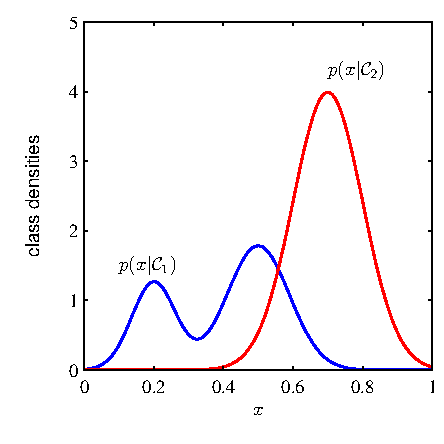
\includegraphics[width=.5\textwidth]{images/Figure1-27a.pdf}
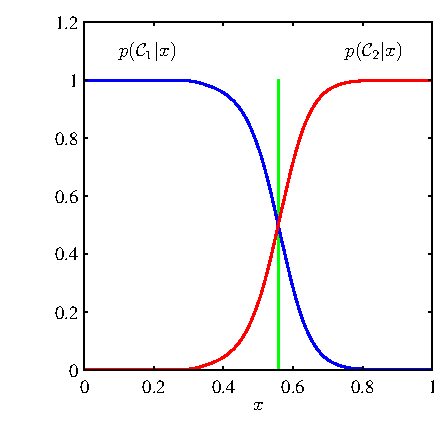
\includegraphics[width=.5\textwidth]{images/Figure1-27b.pdf}
\scriptsize Figure 1.27
(\href{http://research.microsoft.com/en-us/um/people/cmbishop/prml}
{Bishop, 2006}): Example of the class-conditional densities for two
classes having a single input variable $x$ (left plot) together with
the corresponding posterior probabilities (right plot). Note that the
left-hand mode of the class-conditional density $p(x|C_1)$, shown in
blue on the left plot, has no effect on the posterior
probabilities. The vertical green line in the right plot shows the
decision boundary in $x$ that gives the minimum misclassification rate.
\end{frame}

\begin{frame}\frametitle{Conditional log-linear models: Likelihood}
\begin{itemize}
\item Represent $(x, y)$ pairs using a feature vector function
  $\mathbf{g}: \mathcal{X} \times \mathcal{Y} \rightarrow
  \mathbb{R}^d:$ \[
\mathbf{g}(x, y) = [ g_1(x, y), g_2(x, y), \dots, g_d(x, y) ]^T
\]
\item Define score as linear combination of feature values: \[
  \score(x, y) = \mathbf{w}^T \mathbf{g}(x, y) = \sum w_i g_i(x, y)
\]
\item Maximizing score equivalent to maximizing conditional log-linear
  likelihood:
\begin{eqnarray*}
  p_w(y|x) &=& \frac{1}{z_w(x)}\exp \mathbf{w}^T \mathbf{g}(x, y) \\
  z_w(x) &=& \sum_{y'\in\mathcal{Y}} \exp \mathbf{w}^T \mathbf{g}(x, y') \\
  \argmax_{y\in\mathcal{Y}} p_w(y|x)
    &=& \argmax_{y\in\mathcal{Y}} \exp \mathbf{w}^T \mathbf{g}(x, y) \\
    &=& \argmax_{y\in\mathcal{Y}} \mathbf{w}^T \mathbf{g}(x, y)
\end{eqnarray*}
\end{itemize}
\end{frame}

\begin{frame}\frametitle{Conditional log-linear models: What features?}
A typical feature set for string classification (inspired by Naive
Bayes parameters):\begin{itemize}
\item One binary feature for each class:\[
g_j(x, y) = 
\begin{cases}
1,& \text{if } y=j \\
0,& \text{otherwise.}
\end{cases}
\]
\item One binary feature for each word-class pair:\[
g_{ij}(x, y) = 
\begin{cases}
1,& \text{if word}_i\in x, y=j \\
0,& \text{otherwise.}
\end{cases}
\]
\end{itemize}
Typically each feature should be sensitive to the class (a feature
that only looks at $x$ would not be useful in modeling $p(y|x)$), and
possibly some properties of the input string $x$.
\end{frame}

\begin{frame}\frametitle{Conditional log-linear models: MLE}
Given training data $\{(x_1, y_1), (x_2, y_2), \dots \}$, the
maximum likelihood estimation for weights $\mathbf{w}$: \begin{eqnarray*}
\mathbf{w^*} &=& \argmax_\mathbf{w} \prod p_\mathbf{w}(y_i | x_i) \\
&=& \argmax_\mathbf{w} \sum \log p_\mathbf{w}(y_i | x_i) \\
&=& \argmax_\mathbf{w} \sum \mathbf{w}^T \mathbf{g}(x_i, y_i) - \log z_w(x_i)
\end{eqnarray*}
\begin{itemize}
\item There is no closed form solution.
\item The function is concave (unique maximum).
\item Algorithms like LBFGS can find the maximum quickly given the
  gradient.
\end{itemize}
\end{frame}

\begin{frame}\frametitle{Conditional log-linear models: Gradient}
\begin{eqnarray*}
\ell(\mathbf{w}) &=& \frac{1}{N} \sum_{i=1}^N \left[ \mathbf{w}^T
    \mathbf{g}(x_i, y_i) - \log z_w(x_i) \right] \\
\frac{\partial \ell(\mathbf{w})}{\partial w_j} &=& \frac{1}{N}
  \sum_{i=1}^N \left[ g_j(x_i, y_i) - \frac{\sum_{y'\in\mathcal{Y}}
      g_j(x_i, y') \exp \mathbf{w}^T \mathbf{g}(x_i, y')}{z_w(x_i)}
    \right] \\
&=& \frac{1}{N} \sum_{i=1}^N \left[ g_j(x_i, y_i) -
    \sum_{y'\in\mathcal{Y}} g_j(x_i, y') p_w(y'|x_i) \right] \\
&=& \frac{1}{N} \sum_{i=1}^N \left[ g_j(x_i, y_i) -
    \mathbb{E}_{p_\mathbf{w}(Y|X)} g_j(x_i ,Y) \right] \\
&=& \mathbb{E}_{\tilde{p}(X,Y)} g_j(X,Y) -
  \mathbb{E}_{p_\mathbf{w}(X,Y)} g_j(X,Y)
\end{eqnarray*}
where $p_\mathbf{w}(X,Y) = \tilde{p}(X)p_\mathbf{w}(Y|X)$ and
$\tilde{p}$ denotes empirical distribution (i.e. data frequency).
\end{frame}

\begin{frame}\frametitle{Conditional log-linear models: Feature expectations}
\[
\mathbb{E}_{\tilde{p}(X,Y)} g_j(X,Y) =
  \mathbb{E}_{p_\mathbf{w}(X,Y)} g_j(X,Y)\quad \mbox{ at maximum.}
\]
\begin{itemize}
\item The first expectation is over the empirical distribution
  $\tilde{p}$.
\item The second expectation is over the model distribution $p_w$.
\item At the $\mathbf{w}$ that maximizes the likelihood, the model
  expectation of each feature is equal to the empirical expectation.
\end{itemize}
\end{frame}

\begin{frame}\frametitle{Log-linear models under other names}
\begin{itemize}
\item \textbf{Maximum entropy models:} When we represent data using a
  given set of features and ask for the probability distribution with
  maximum entropy consistent with empiricial feature expectations, the
  log-linear model gives the unique solution.  (Thus they are also
  called maximum entropy models.)
\item \textbf{Logistic regression:} (actually a classification, not a
  regression technique) is a conditional log-linear model for binary
  outputs.
\item \textbf{CRF, MEMM:} Structured conditional log-linear models (to
  be covered later).
\item \textbf{Naive Bayes:} gives the maximum likelihood solution to a
  {\em generative} log-linear model (modeling joint instead of
  conditional probability as a log-linear function of features)
  i.e. $p_w(x,y) = \frac{1}{z_w}\exp \mathbf{w}^T \mathbf{g}(x, y)$
  (see
  \href{http://www.denizyuret.com/2010/11/naive-bayes-is-joint-maximum-entropy.html}{my
    blog post on this}).
%% linear svm vs logistic regression with l1/l2 prior, l1/l2 loss?
\end{itemize}
\end{frame}

\begin{frame}\frametitle{Conditional log-linear models: Overfitting}
%% LSP pp.94
Example from (LSP, pp.94): Consider a feature $g_6$ with value 1 on a
single training example $(x_9, y_9)$ and 0 for every other $(x, y)$
pair.  The derivative of the log likelihood with respect to $w_6$
is: \begin{eqnarray*} \frac{\partial \ell(\mathbf{w})}{\partial w_6}
  &=& \frac{1}{N} \sum_{i=1}^N \left[ g_6(x_i, y_i) -
    \sum_{y'\in\mathcal{Y}} g_6(x_i, y') p_\mathbf{w}(y'|x_i) \right]
  \\ &=& \frac{1}{N} \left[g_6(x_9, y_9) - g_6(x_9, y_9)
    p_\mathbf{w}(y_9|x_9)\right] \\ &=& \frac{1}{N} \left[ 1 -
    p_\mathbf{w}(y_9|x_9) \right]
\end{eqnarray*}
This derivative can only approach 0 if $p_\mathbf{w}(y_9|x_9)$
approaches 1.\begin{eqnarray*}
p_\mathbf{w}(y_9|x_9) &=& \frac{\exp \mathbf{w}^T \mathbf{g}(x_9,y_9)}
{\sum_{y'\in\mathcal{Y}} \exp \mathbf{w}^T \mathbf{g}(x_9,y')} \\
\end{eqnarray*}
This can only happen if $w_6\rightarrow\infty$ and for every feature
$g_j$ involving a competing $y'$, $w_j\rightarrow-\infty$.
\end{frame}

\begin{frame}\frametitle{MAP estimation as a solution to overfitting}
\begin{itemize}
\item Predictive distribution (what we really want):\begin{eqnarray*}
  P(D'|D,\mathcal{H}) &=& \int P(D'|Q,\mathcal{H}) P(Q|D,\mathcal{H}) dQ \\
  \text{where } P(Q|D,\mathcal{H}) &\propto& P(D|Q,\mathcal{H}) P(Q|\mathcal{H})
\end{eqnarray*}
\item Maximum likelihood estimate (MLE):\begin{eqnarray*}
  P(D'|D,\mathcal{H}) &\approx& P(D'|Q_\text{ML}, \mathcal{H}) \\
\mbox{where } Q_\text{ML} &=& \argmax_Q P(D|Q,\mathcal{H})
\end{eqnarray*}
\item Maximum a-posteriori estimate (MAP):\begin{eqnarray*}
  P(D'|D,\mathcal{H}) &\approx& P(D'|Q_\text{MAP}, \mathcal{H}) \\
\mbox{where } Q_\text{MAP} &=& \argmax_Q P(Q|D,\mathcal{H}) \\
\mbox{ and } P(Q|D,\mathcal{H}) &\propto& P(D|Q,\mathcal{H}) P(Q|\mathcal{H})
\end{eqnarray*}
\end{itemize}
\footnotesize Note: In generative models $D$ and $D'$ stand for both
the input $X$ and the output $Y$.  In conditional models they stand
for the output $Y$ only.  The input $X$ is assumed given ($X$ is on
the condition (right) side of each probability).
% expression, next to $\mathcal{H}$).
\end{frame}

\begin{frame}\frametitle{Conditional log-linear models: Gaussian MAP} %% LSP 94-97
Gaussian prior (aka L2 regularization):\begin{eqnarray*}
p(\mathbf{w}|\mathcal{H}_G) &=& \prod_{j=1}^d \frac{1}{\sigma \sqrt{2\pi}}
\exp -\frac{w_j^2}{2\sigma^2} \\
\mathbf{w}_\text{MAP} &=& \argmax_w\, \log p(D|\mathbf{w},\mathcal{H}_G)
+ \log p(\mathbf{w}|\mathcal{H}_G) \\
&=& \argmax_w\, \ell(\mathbf{w}) -\frac{1}{2\sigma^2}\sum w_j^2 \\
&=& \argmax_w\, \ell(\mathbf{w}) - \frac{C}{2}\|\mathbf{w}\|_2^2 \quad\text{where }C=\frac{1}{\sigma^2}
\end{eqnarray*}
\end{frame}
\begin{frame}\frametitle{Conditional log-linear models: Laplacian MAP} %% LSP 94-97
Laplacian prior (aka L1 regularization):\begin{eqnarray*}
p(\mathbf{w}|\mathcal{H}_L) &=& \prod_{j=1}^d \frac{1}{2b} \exp -\frac{|w_j|}{b}\\
\mathbf{w}_\text{MAP} &=& \argmax_w\, \log p(D|\mathbf{w},\mathcal{H}_L)
+ \log p(\mathbf{w}|\mathcal{H}_L) \\
&=& \argmax_w\, \ell(\mathbf{w}) -\frac{1}{b}\sum |w_j| \\
&=& \argmax_w\, \ell(\mathbf{w}) - C \|\mathbf{w}\|_1 \quad\text{where }C=\frac{1}{b}
\end{eqnarray*}
\end{frame}

\begin{frame}\frametitle{Conditional log-linear models: L1 vs. L2} %% Hastie
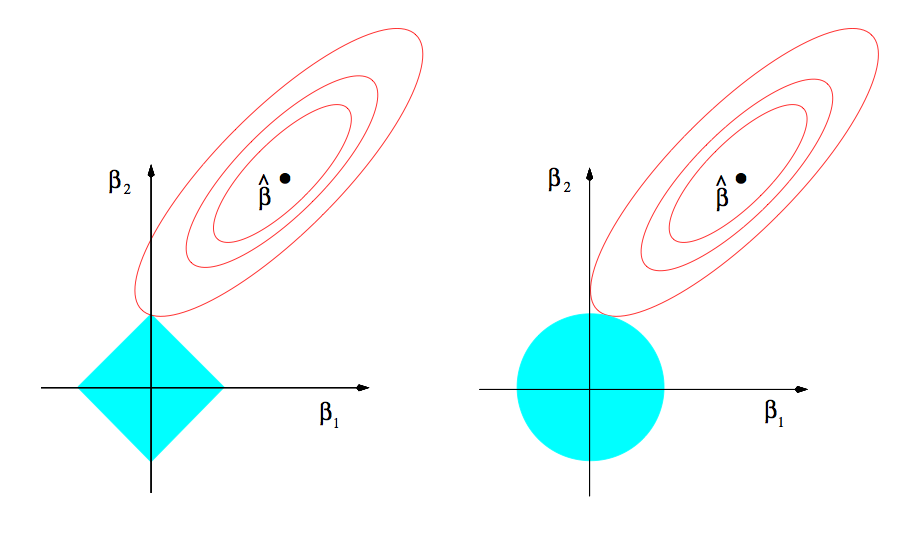
\includegraphics[width=.9\textwidth]{images/hastie-fig-3-11.png}

\footnotesize Adapted from (Hastie et al. 2011, Fig 3.11): $\beta_1$
and $\beta_2$ are model parameters, $\hat{\beta}$ is the ML estimate,
the red ellipses are likelihood contours, and the solid blue shapes
are the L1 (left) and L2 (right) prior contours.  The L1 prior results
in a more sparse (with lots of zeros) parameter vector.  The L2 prior
pushes many parameters close to zero but does not quite get rid of
them.
\end{frame}

\begin{frame}\frametitle{A non-probabilistic view of learning} %% LSP 98-100
\begin{itemize}
\item An alternative view of machine learning replaces probabilistic
inference with the minimization of a {\bf loss function}.  
\item Let $\mathcal{H}$ denote the set of all possible predictors that
  map $\mathcal{X}\rightarrow\mathcal{Y}$.  
\item The loss for $h\in\mathcal{H}: \loss(\mathbf{x}, \mathbf{y}; h)$
  measures the badness of the predictor $h$ given input $\mathbf{x}$
  when $\mathbf{y}$ is the correct output.
\item Given $\mathcal{H}$ and $\loss$, the learning problem becomes:\[
  \min_{h\in\mathcal{H}} \mathbb{E}[\loss(\mathbf{X}, \mathbf{Y}; h)]
  + \textit{model-complexity}(h)
\]
\item The second term takes the place of the prior and is called the
  {\bf regularization} term.
\item When the expected loss is approximated using the sample
  distribution we have what is called the {\bf empirical risk}:\[
  \mathbb{E}[\loss(\mathbf{X}, \mathbf{Y}; h)] \approx \frac{1}{N}
  \sum_{i=1}^N \loss(x_i, y_i; h)
\]
\end{itemize}
\end{frame}

\begin{frame}\frametitle{Probabilistic inference $\equiv$ log loss}
The probabilistic learning methods we have covered can be restated in
terms of loss functions.
\begin{itemize}
\item Maximizing log likelihood in generative models can be seen as
  minimizing the {\bf log loss}:\[
\loss(x, y; h) = -\log p(x, y | h)
\]
\item Maximizing log likelihood in conditional models gives another
  form of {\bf log loss}:\[
\loss(x, y; h) = -\log p(y | x, h)
\]
\end{itemize}
\end{frame}
\begin{frame}\frametitle{Potential problems with log loss}
\begin{eqnarray*}
\loss(x, y; h) &=& -\log p(x, y | h)\quad\text{or}\\
\loss(x, y; h) &=& -\log p(y | x, h)
\end{eqnarray*}
\begin{itemize}
\item Even if the model correctly predicts $y_i$ as the most probable
  output for $x_i$, there is still pressure to diminish the loss
  function as long as other $y\in\mathcal{Y}$ have non-zero
  probability.
\item Not all alternative $y\in\mathcal{Y}$ may be equally bad, some
  wrong answers may be preferrable to others.  This is not represented
  in log loss.
\end{itemize}
\end{frame}

\begin{frame}\frametitle{Alternative loss functions}
\begin{center}
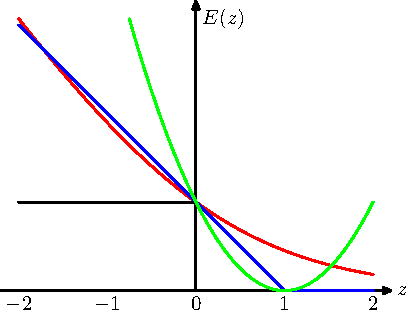
\includegraphics[height=.5\textheight]{images/bishop-fig-7-5.pdf}
\end{center}\footnotesize
{\bf Figure 7.5 (from Bishop, 2006)}: Loss functions for binary
classification $y\in\{-1,+1\}$.  $z=y\hat{y}$ where $y$ is the correct
output and $\hat{y}$ is the model output.  $E(z)$ gives the loss (or
error) for a single instance.  The red curve is equivalent to {\bf
  log-loss}, the black curve is {\bf 0-1 loss}, the blue curve is {\bf
  hinge loss} (used by SVM), and the green curve is the {\bf squared
  error} loss.  Each loss function may imply different optimum
parameters for a given model.
\end{frame}

\begin{frame}\frametitle{Perceptron} %% LSP 101-103

\end{frame}

\begin{frame}\frametitle{SVM} %% LSP 103-104

\end{frame}

\end{document}
